\begin{figure*}[tb]

{\centering 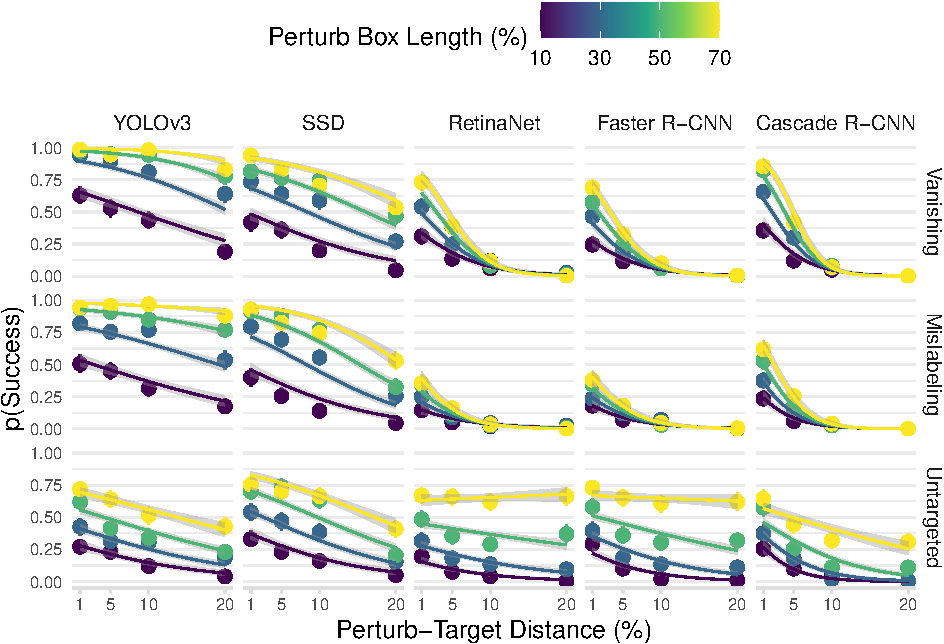
\includegraphics[width=1\linewidth]{imgs/arbitrary_trend_graph-1} 

}

\caption{Perturbing an arbitrary region obfuscates intent with increased success for all models and attacks:  We implement intent obfuscating attack by perturbing an arbitrary non-overlapping square region to disrupt a randomly selected target object at various lengths and distances. The binned summaries and regression trendlines graph success proportion against perturb-target distance and perturb box length, both relative to image width or height, in the deliberate attack experiment. Errors are 95\% confidence intervals and every point aggregates success over 200 images. The deliberate attack multiplies success as compared to the randomized attack (Figure \ref{fig:success_trend_graph}), especially at close perturb-target distance and large perturb box length. Full details are given in Section \ref{sec:del_arb}.}\label{fig:arbitrary_trend_graph}
\end{figure*}